\documentclass[twocolumn,a4paper]{article}
\usepackage{graphicx}
\usepackage{subfigure}
\usepackage{amsfonts}
\usepackage{color}
\usepackage{lineno}
\setlength{\columnsep}{10pt}
\setlength{\oddsidemargin}{0pt}
\setlength{\topmargin}{0pt}
\setlength{\headheight}{0pt}
\setlength{\headsep}{0pt}
\setlength{\marginparsep}{0pt}
\setlength{\marginparwidth}{0pt}
\addtolength{\voffset}{-50pt}
\setlength{\textheight}{26.8cm}
\author{Siwang Li}

\title{RS update}

%% document begin here
\begin{document}
\maketitle

\section{Introduction}
For simplicity of implementation, I used much simpler scheme than the approach
TVCG to update the inverted rotation axis when computing $log(R)$. I found that
the RS coordinates of the last frame $y_{T}$ is very similar to the ground truth
coordinates $y'_T$. Thus, for each tetrahedron $e$, I compare the rotational
vector $w_f=y^e_{f}$ and $w_{f+1}=y^e_{f+1}$ for $f\in[0,T-1]$, if
$w_f^Tw_{f+1}<-0.5$, I will update $w_f$ using
\begin{equation}
  w_f = \frac{w_f}{\|w_f\|_2}(\|w_f\|_2-2\pi)
\end{equation}
The resulting $z_i$ are shown in figure \ref{zzc}.
\begin{figure}
  \centering
  \subfigure[mode 1,2,3] { \label{fig:a} 
  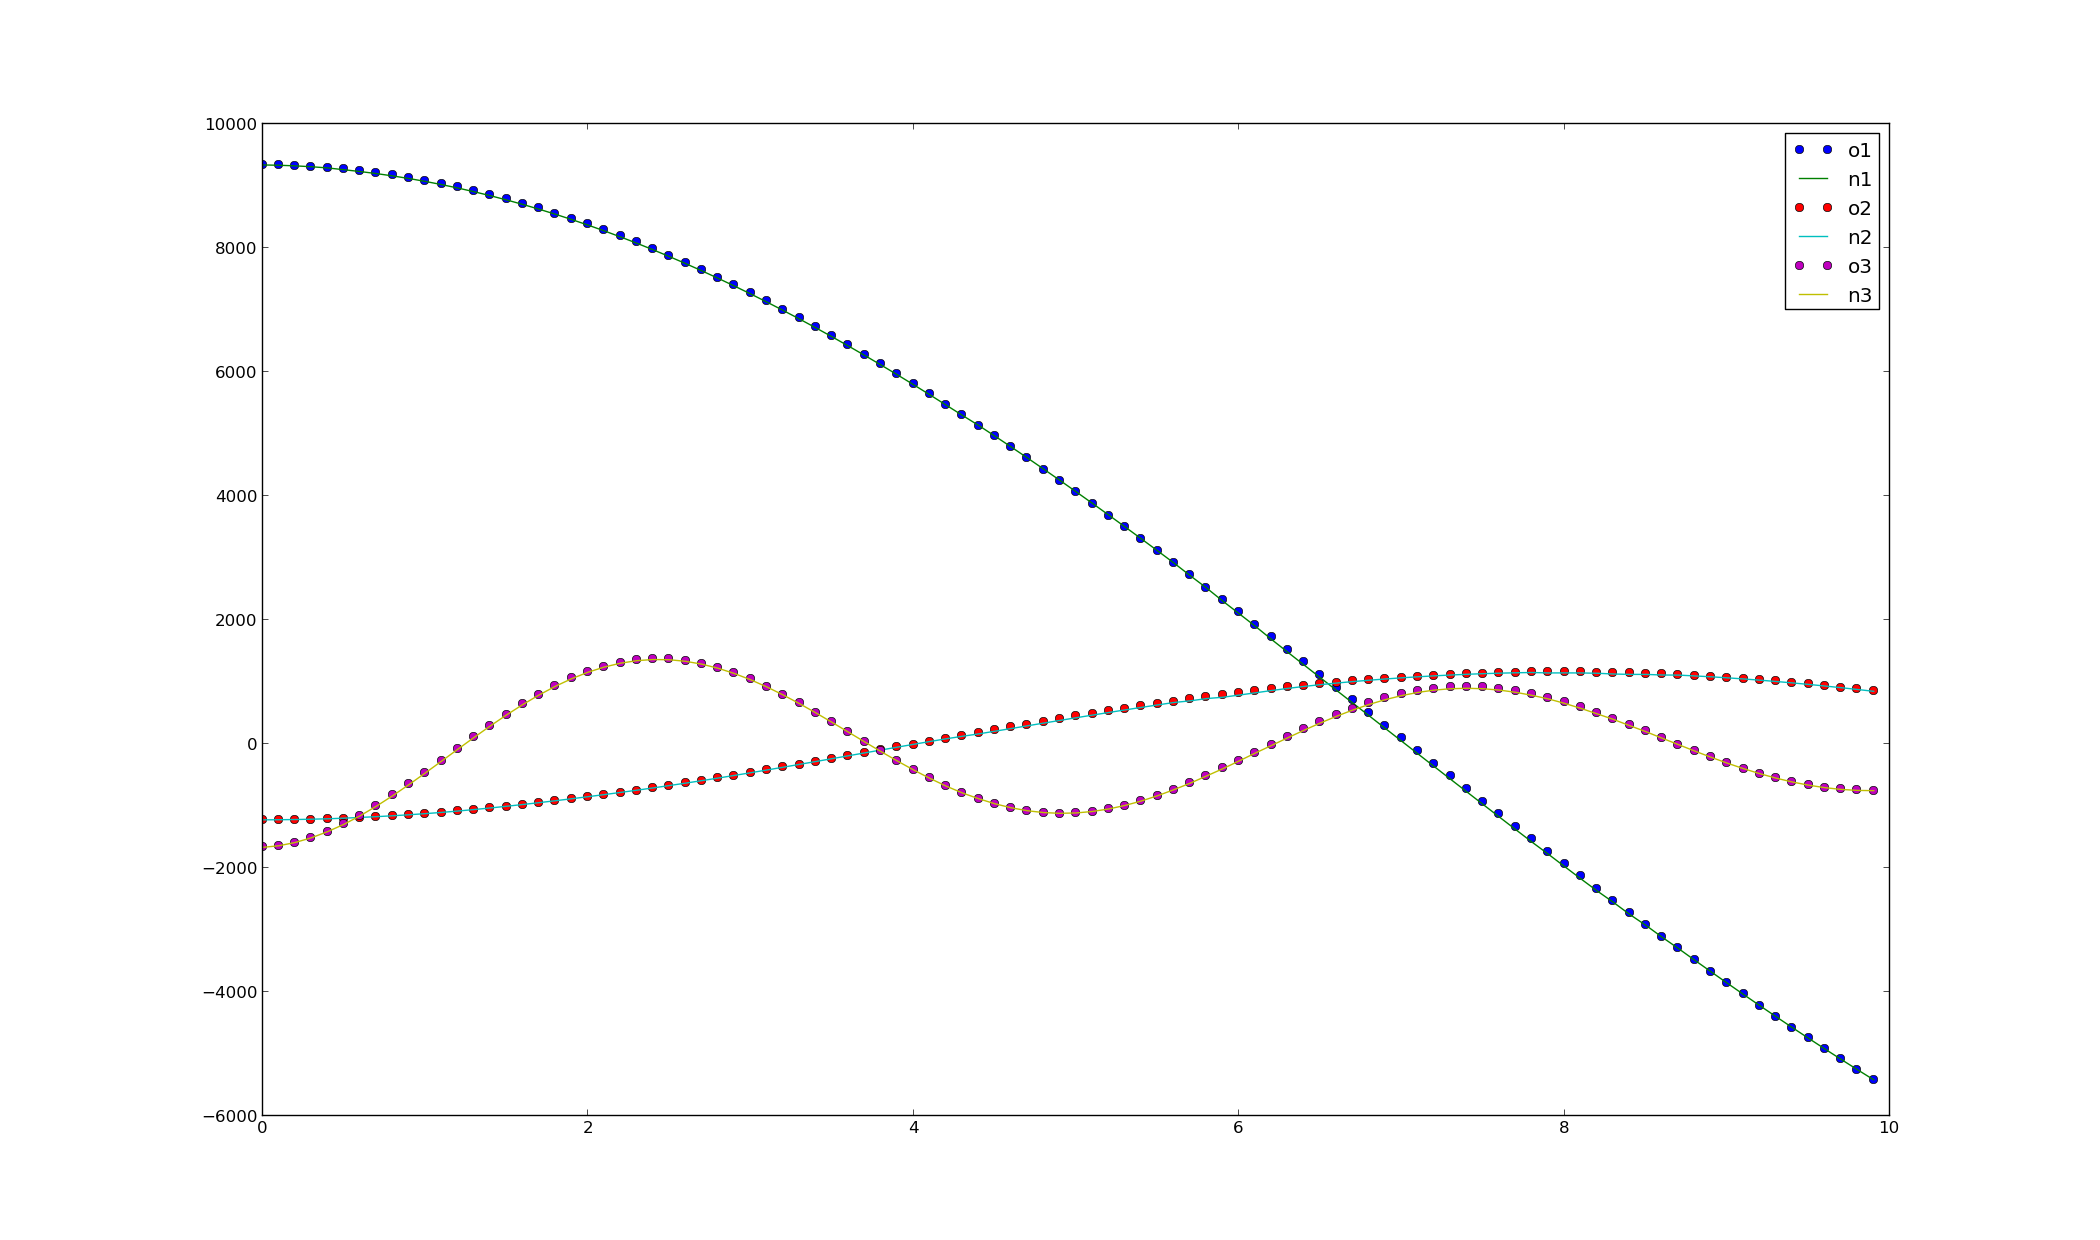
\includegraphics[width=0.48\textwidth]{./figures/uprs1.png}
  }
  \subfigure[mode 4,5,6] { \label{fig:b} 
  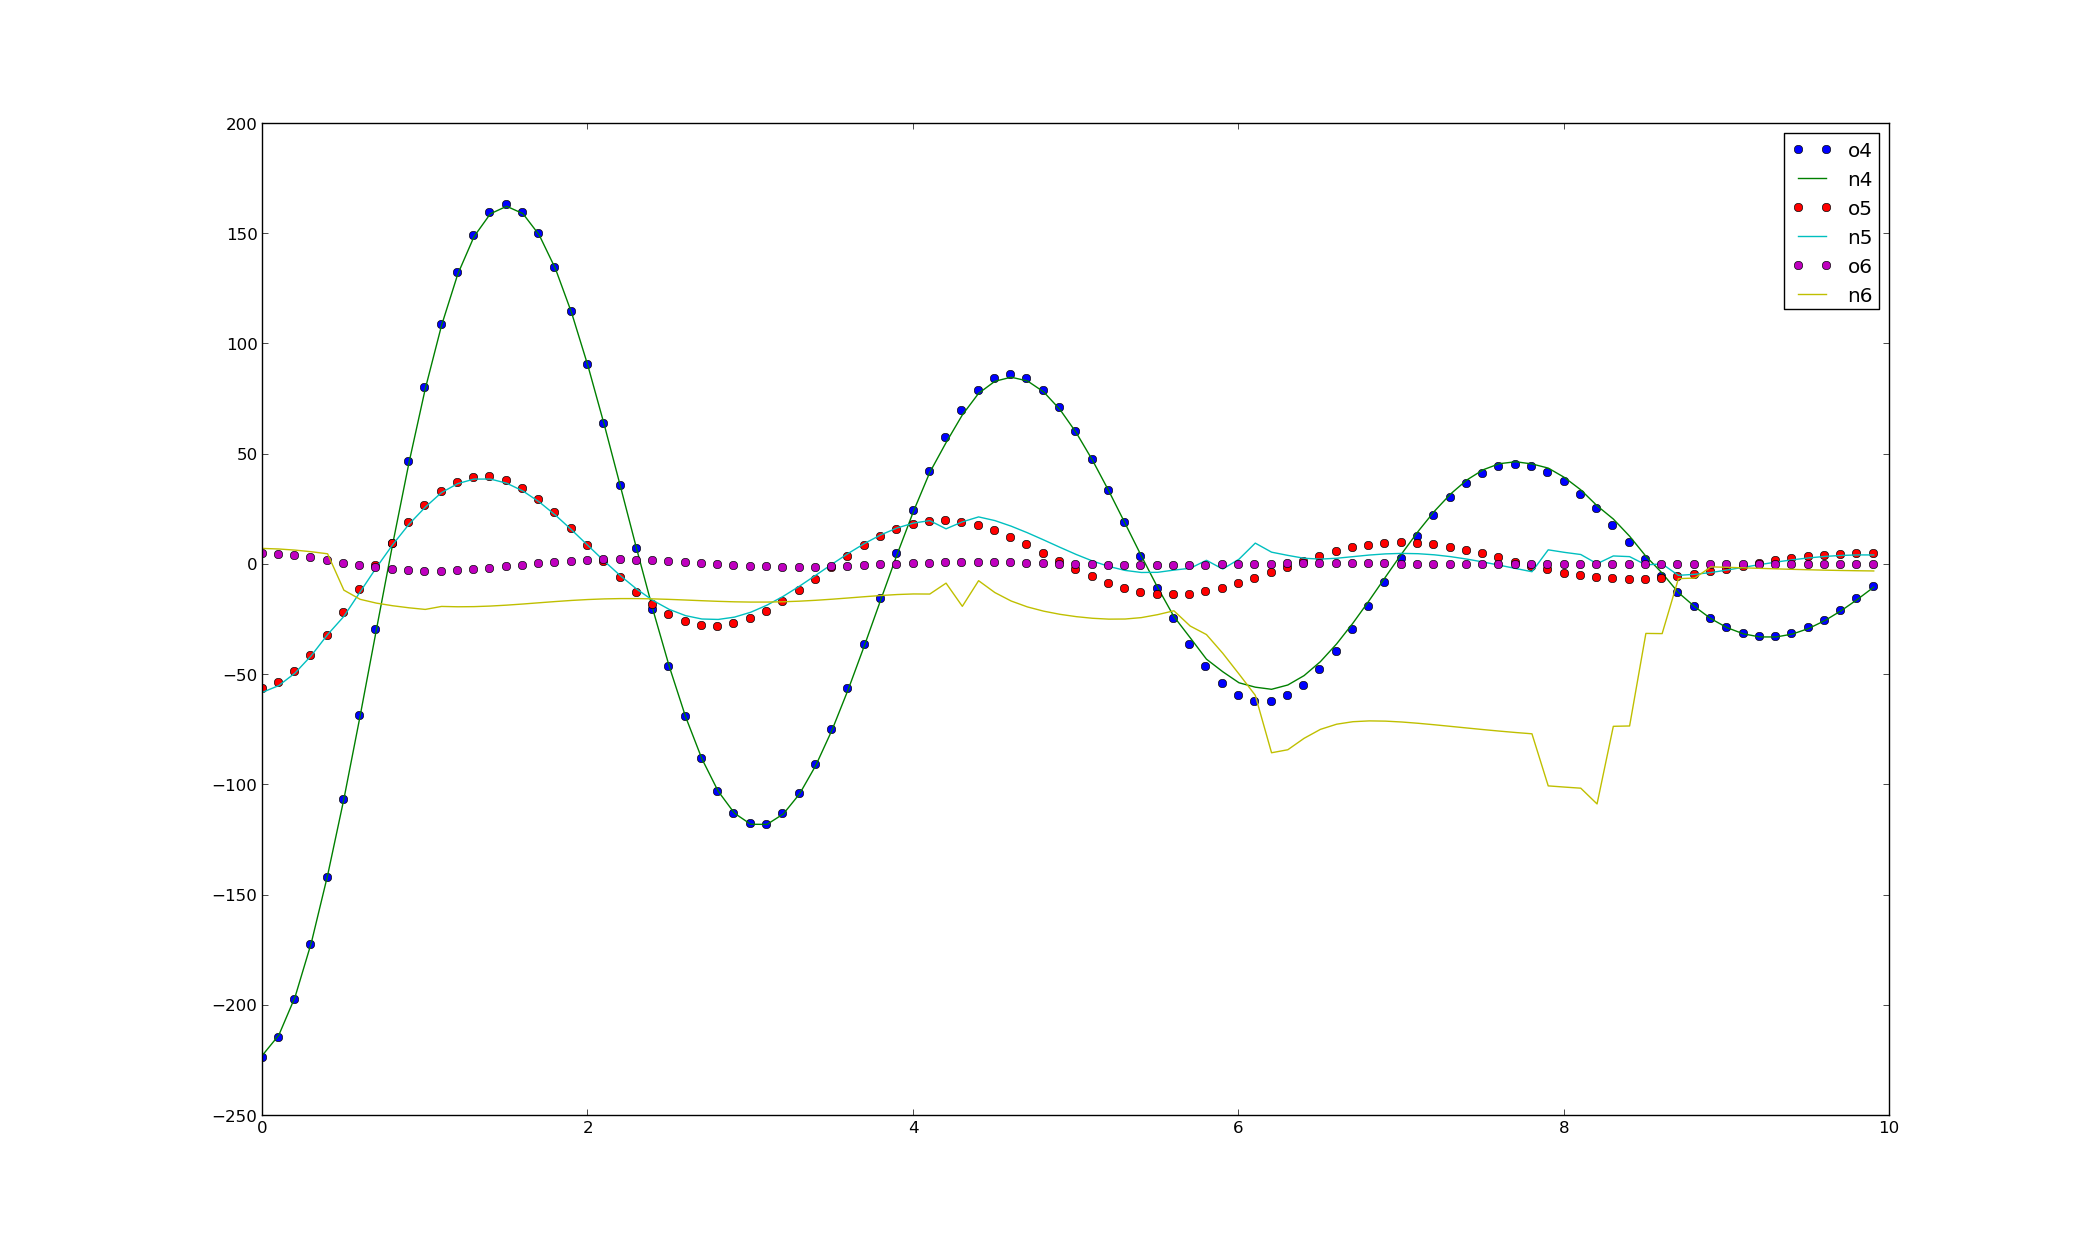
\includegraphics[width=0.48\textwidth]{./figures/uprs2.png}
  }
  \subfigure[mode 7,8,9] { \label{fig:b} 
  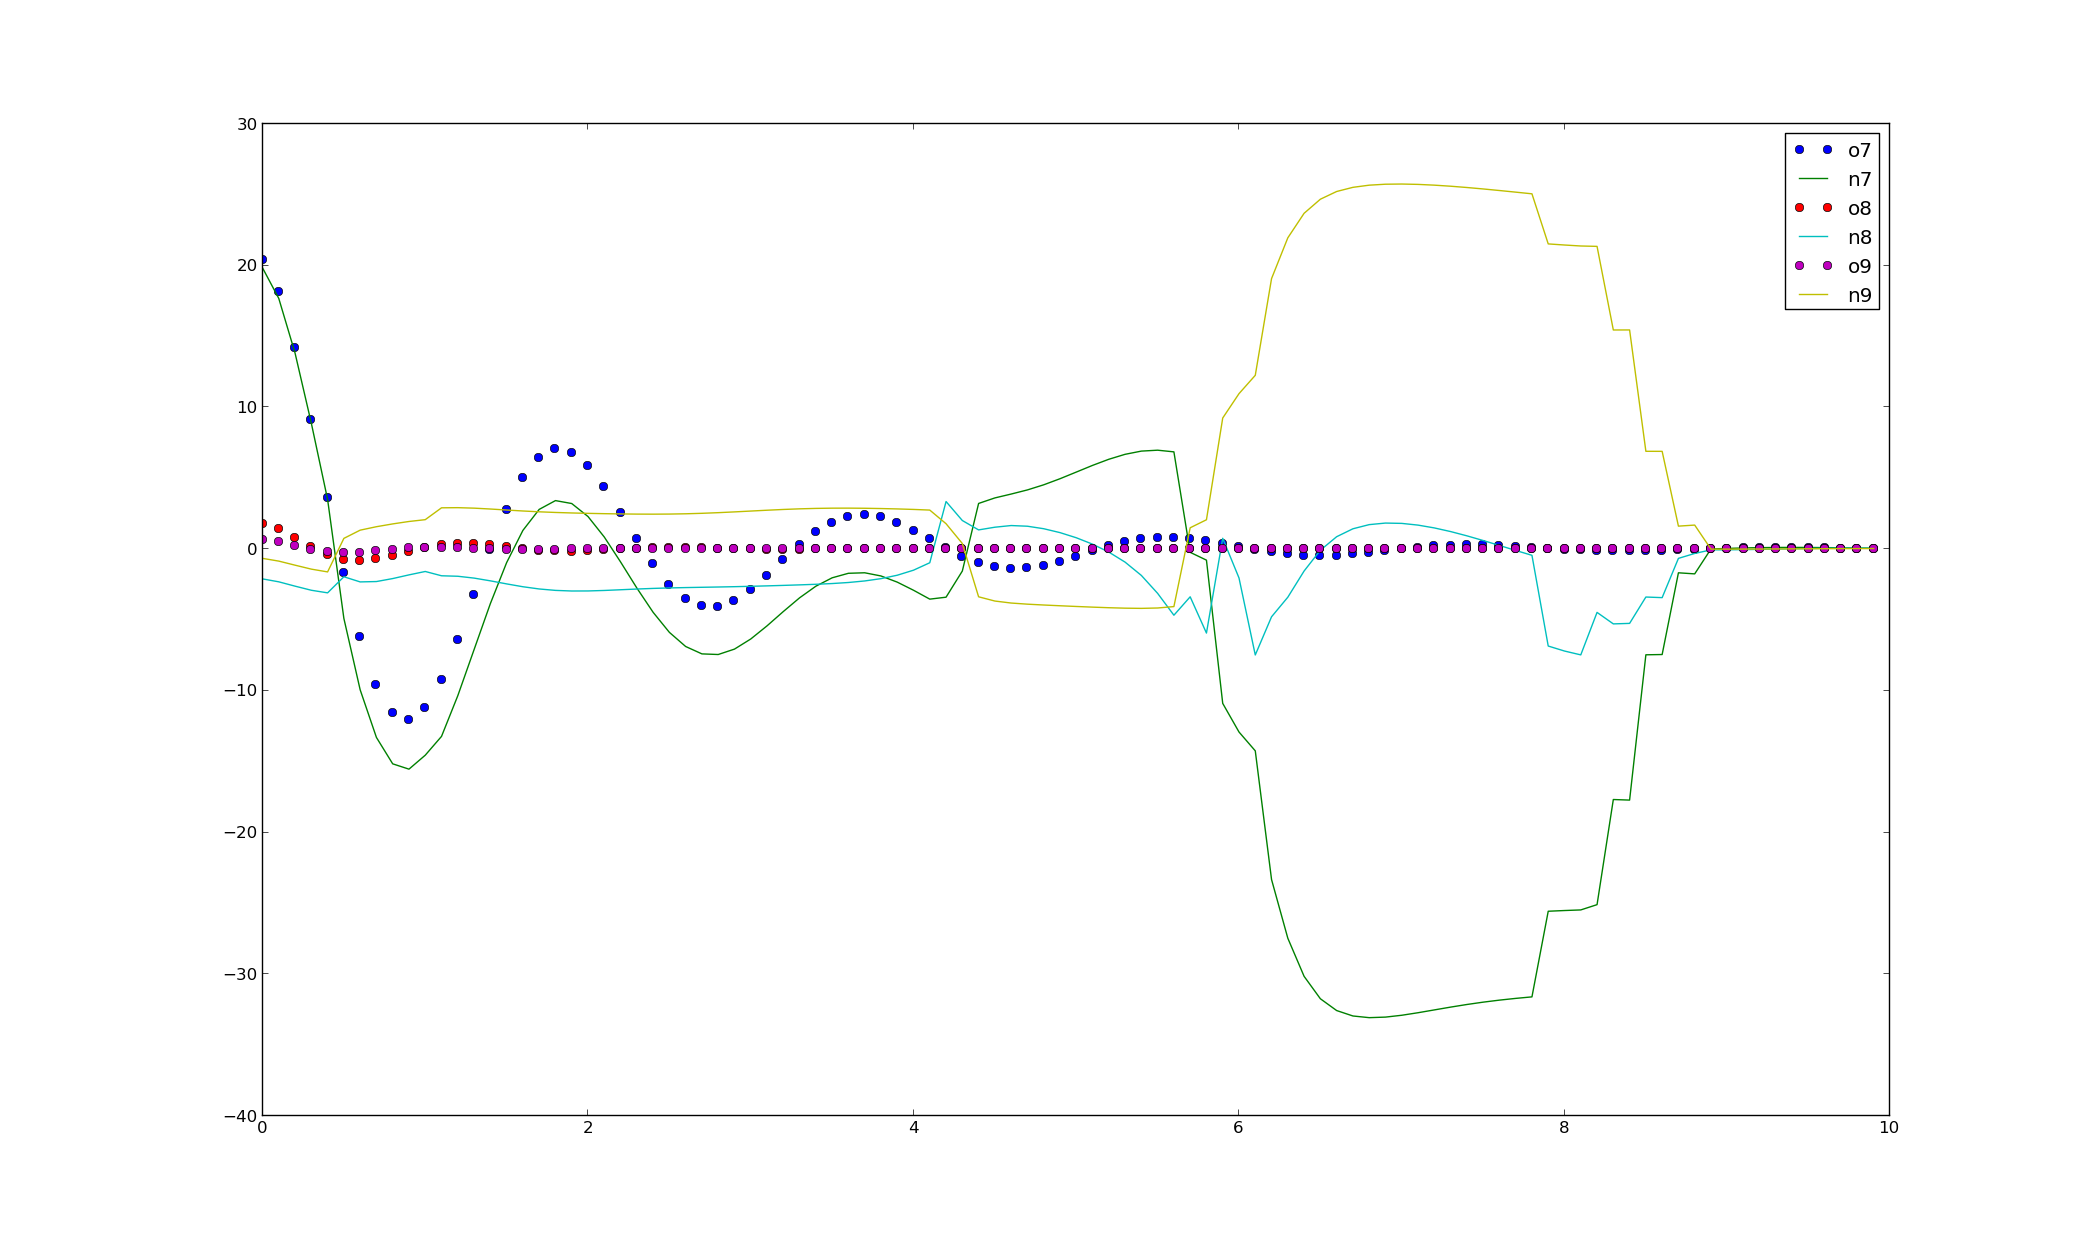
\includegraphics[width=0.48\textwidth]{./figures/uprs3.png}
  }
  \caption{Points are $z$, and others are $z'$. Time step is $0.1$, and there is
    100 frames here.}
  \label{zzc}.
\end{figure}

\end{document}
